\section{The First Machine: A Traffic Light Controller}
\label{tut_first_machine}

% a first machine, e.g. a traffic light with booleans for signals.  We introduce guards, resulting in the proof obligations to be discharged automatically. We explain how proof lables are read, without changing to the proof perspective.

\tick{\textbf{Goals:} The objective of this section is to get acquainted with the modeling environment. We will create a very simple model consisting of just one file to develop a feeling for Rodin and Event-B.}

In this tutorial, we will create a model of a traffic light controller.  We will use this example repeatedly in subsequent sections.  Figure \ref{fig_tut_03_traffic_light} depicts what we are trying to achieve.

\begin{figure}[!ht]
\begin{center}
	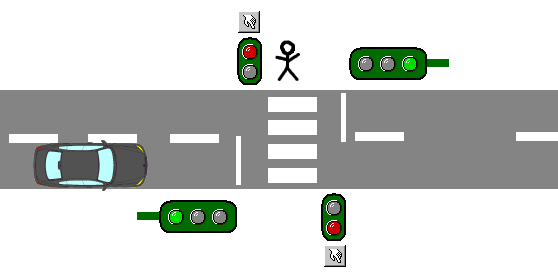
\includegraphics[]{img/tutorial/tut_03_trafficlight.png}
	\caption{The traffic light controller}
	\label{fig_tut_03_traffic_light}
\end{center}
\end{figure}

In this section, we will implement a simplified controller with the following characteristics:
\begin{itemize}
	\item We will model the signals with boolean values to indicate ``stop'' (false) and ``go'' (true).  We do not model colors (yet) because
      we think we should first specify our goal (regulating the traffic) and later we should add implementation details (the traffic light's colors).
	\item Too keep the initial model simple, we will not include the push button yet. We will add it later.
\end{itemize}

\subsection{Excursus: The specification process}
\label{tut_excursus_the_sepcification_process}

While this handbook is concerned with use of the Rodin tool, it's important to understand the specification process as well.  Especially for beginners it can be daunting and unclear where to start with the model, what kind of data structures and abstractions to use, and so on.

We cover a few examples in this chapter that implicitly answer these questions, but there is no explicit set of instructions.  For example, we will first model the traffic lights as booleans, and later refine them into actual colors.  But how did we come up with this refinement strategy?  Likewise, we decided to add the push buttons at a later refinement.  In retrospect this may seem useful, but it leaves open the question on how we arrived at this structure in the first place.

Abrial has something to say about this in his book\footnote{\url{http://www.amazon.com/Modeling-Event-B-System-Software-Engineering/dp/0521895561}}, for which some chapters are available in the Rodin Wiki.

\subsection{Project Setup}
\label{tut_project_setup}

Models typically consist of multiple files that are managed in a project.  Create a new Event-B Project \textsf{File $\rangle$ New $\rangle$ Event-B Project}.  Give the project the name \texttt{tutorial-03} as shown in Figure \ref{fig_tut_03_new_project_wizard}.

\begin{figure}[!ht]
\begin{center}
	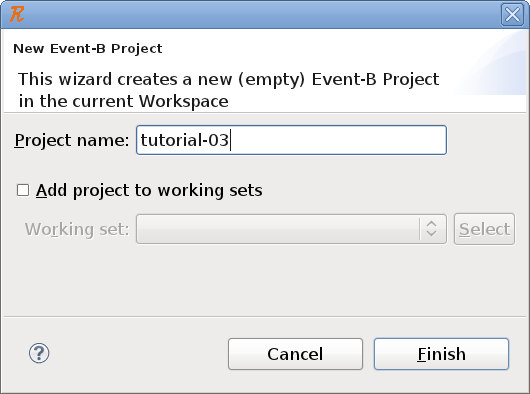
\includegraphics[]{img/tutorial/tut_03_tutorial-3.png}
	\caption{New Event-B Project Wizard}
	\label{fig_tut_03_new_project_wizard}
\end{center}
\end{figure}

\index{project}
\warning{Eclipse supports different types of projects.  The project must have the Rodin Nature (\ref{rodin_nature}) to work.  A project can have more than one nature.}

\index{component}
Next, create a new Event-B Component.  Either use \textsf{File $\rangle$ New $\rangle$ Event-B Component} or right-click on the newly created project and select \textsf{New $\rangle$ Event-B Component}.  Use \texttt{mac} as the component name, select \textsf{Machine} as component-type, and click \textsf{Finish} as shown in Figure \ref{fig_tut_03_new_component_wizard}. This will create a Machine (\ref{machine}) file.

\begin{figure}[!ht]
\begin{center}
	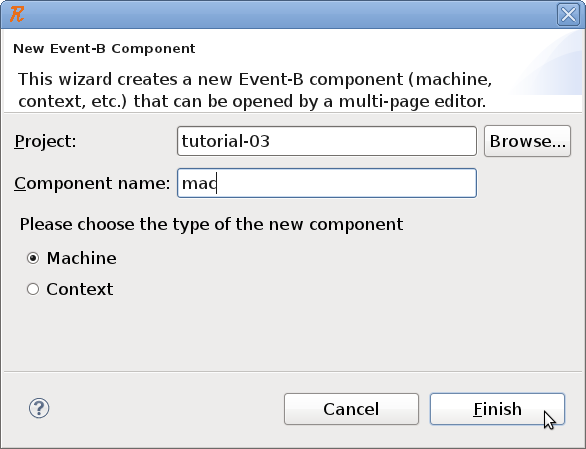
\includegraphics[]{img/tutorial/tut_03_mac.png}
	\caption{New Event-B Component Wizard}
	\label{fig_tut_03_new_component_wizard}
\end{center}
\end{figure}

The newly created component will open in the structural editor.  The editor has four tabs at the bottom.  The \textsf{Pretty Print} shows the model as a whole with color highlighting, but it cannot be edited here.  This is useful to inspect the model.  The \textsf{Edit} allows editing of the model.  It shows the six main sections of a machine (REFINES, SEES, etc.) in a collapsed state.  You can click on the \icon{rodin/collapsed.png} button to the left of a section to expand it.

%\begin{figure}[!ht]
%\begin{center}
%	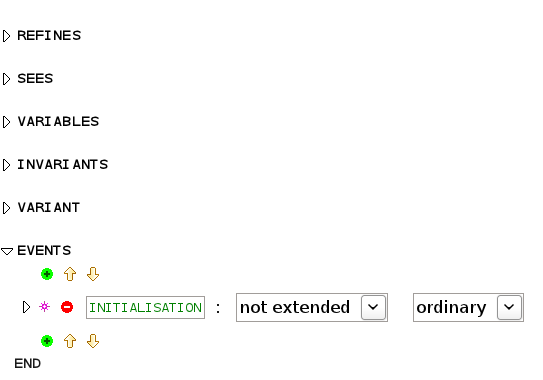
\includegraphics[]{img/tutorial/tut_03_interface.png}
%\end{center}
%\end{figure}

The editor is \textit{form-based}.  This means that in well-defined places an appropriate control (text field, dropdown, etc.) allows modifications.

\info{Alternative editors are available as plug-ins.  The form editor has the advantage of guiding the user through the model, but it takes up a lot of space and can be slow for big models.  The text-based Camille Editor (\ref{tut_camille}) is very popular.  Please visit the Rodin Wiki (\ref{rodin_wiki}) for the latest information.}

\subsection{Camille, a text-based editor}
\label{tut_camille}
\begin{rodin-plugin}{img/camille.png}{Camille}
Camille is a ``real'' text editor that provides the same feel as a typical Eclipse text editor, including copy and paste, undo, redo, etc.  However, please note that at this time, not all Rodin plugins are compatible with Camille.  Also, please consult the extensive documentation in the Rodin Wiki (\ref{rodin_wiki}).

Camille can be installed via its update site, which is preconfigured in Rodin.  Once installed, Camille is made the default editor.  The structural editor can still be used by selecting it from the context menu of a file in the project browser.

For more information, please visit \url{http://wiki.event-b.org/index.php/Text_Editor}.


\end{rodin-plugin}

\subsection{Building the Model}
\label{tut_building_the_model}

Back to the problem: Our objective is to build a simplified traffic light controller as described in \ref{tut_first_machine}.  We start with the model state.  Two traffic lights will be modelled and we will therefore create two variables called  \texttt{cars\_go} and \texttt{peds\_go}.  

\subsubsection{Creating Variables}
\index{variable!creating a variable}
Go to the \textsf{Edit} tab in the editor and expand the \textsf{VARIABLES} section.  Click on the \icon{rodin/add.png} button to create a new variable.
You will see two fields. The left one is filled with the word \texttt{var1}.  Change this to \texttt{cars\_go}.  The second field (after the double-slash ``//'') is a comment field in which you can write any necessary notes or explanations.

\index{comment}
\info{\textbf{Comments:} The comment field supports line breaks.  Note that it is not possible to ``comment out'' parts of the model, as is possible with most programming languages.  You can use the comment field to ``park'' predicates and other strings temporarily.}

Create the second variable (\texttt{peds\_go}) in the same way.

%\begin{figure}[!ht]
%\begin{center}
%	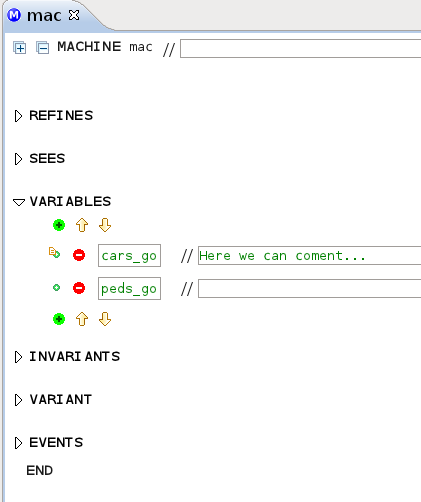
\includegraphics[]{img/tutorial/tut_03_new-variable.png}
%\end{center}
%\end{figure}

Upon saving, the variables will be highlighted in red, indicating an error as shown in Figure \ref{fig_tut_03_error}.  The \textsf{Rodin Problems} view (\ref{rodin_problems_view}) shows corresponding error messages. In this case, the error message is ``Variable cars\_go does not have a type''.

\begin{figure}[!ht]
\begin{center}
	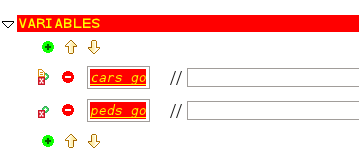
\includegraphics[]{img/tutorial/tut_03_error.png}
	\caption{Red highlighted elements indicate errors}
	\label{fig_tut_03_error}
\end{center}
\end{figure}

Types are provided by invariants. Expand the \textsf{INVARIANTS} section and add two elements by following the same steps as above.  Invariants have labels.  Default labels are generated (\texttt{inv1} and \texttt{inv2}).  The actual invariant is prepopulated with $\btrue$, which represents the logical value ``true''.
Change the first invariant (the $\btrue$, not the label \texttt{inv1}) to $cars\_go \in  BOOL$ and the second invariant to $peds\_go \in  BOOL$.
Event-B provides the build-in datatype \texttt{BOOL} amongst others (\ref{data_types}).

%\begin{figure}[!ht]
%\begin{center}
%	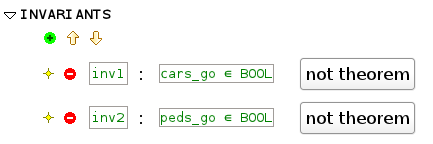
\includegraphics[width=0.7\textwidth]{img/tutorial/tut_03_invariants.png}
%\end{center}
%\end{figure}

\info{\textbf{Mathematical Symbols:} Every mathematical symbol has an ASCII-representation and the substitution occurs automatically.  To generate ``element of'' ($\in$), simply type a colon (``:'').  The editor will perform the substitution after a short delay. The \textsf{Symbols} view shows all supported mathematical symbols. The ASCII representation of a symbol can be found by hovering over the symbol in question.}

\index{yellow highlighting}
After saving, you should see that the \textsf{EVENTS} section is highlighted in yellow as demonstrated in Figure~\ref{fig_tut_03_warning}.  Again, the \textsf{Rodin Problems} view gives us the error message: ``Variable cars\_go is not initialized''. Every variable must be initialized in a way that is consistent with the model.

\begin{figure}[!ht]
\begin{center}
	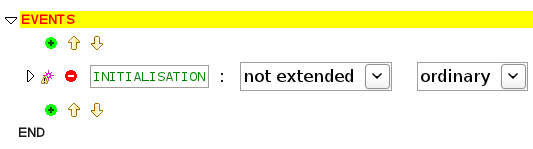
\includegraphics[]{img/tutorial/tut_03_yellow.png}
	\caption{Yellow highlighted elements indicate warnings}
	\label{fig_tut_03_warning}
\end{center}
\end{figure}

To fix this problem, expand the \textsf{EVENTS} section and then the INITIALIZATION event.  Add two elements in the \textsf{THEN} block.  These are actions that also have labels.  In the action fields, enter $cars\_go :=  FALSE$ and $peds\_go :=  FALSE$.

%\begin{figure}[!ht]
%\begin{center}
%	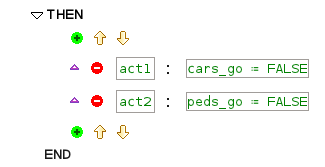
\includegraphics[]{img/tutorial/tut_03_events.png}
%\end{center}
%\end{figure}

\subsubsection{State Transitions with Events}

Our traffic light controller cannot yet change its state.  To make this possible, we create events (\ref{events}). We will first consider the traffic light for the pedestrians, and we will create two events. One will set it to ``go'' and one will set it to ``stop''.

\warning{From now on, we won't describe the individual steps in the editor any more.  Instead, we will simply show the resulting model.} 

The two events will look as follows:

\pencil{
\begin{description}
	\EVT {set\_peds\_go}
		\begin{description}
		\BeginAct
			\begin{description}
			\nItemX{ act1 }{ peds\_go :=  TRUE }
			\end{description}
		\EndAct
		\end{description}
	\EVT {set\_peds\_stop}
		\begin{description}
		\BeginAct
			\begin{description}
			\nItemX{ act1 }{ peds\_go :=  FALSE }
			\end{description}
		\EndAct
		\end{description}
\end{description}
}

\subsubsection{Event parameters}
\index{parameter}

For the traffic light for the cars, we present a different approach and use only one event with a parameter.  The event will use the new traffic light state as the argument.  The parameter is declared in the \textsf{any} section and typed in the \textsf{where} section:

\pencil{
\begin{description}
	\EVT {set\_cars}
		\begin{description}
		\AnyPrm
			\begin{description}
			\ItemX{ new\_value }
			\end{description}
		\WhereGrd
			\begin{description}
			\nItemX{ grd1 }{ new\_value \in  BOOL }
			\end{description}
		\ThenAct
			\begin{description}
			\nItemX{ act1 }{ cars\_go :=  new\_value }
			\end{description}
		\EndAct
		\end{description}
\end{description}
}

Note how the parameter is used in the action block to set the new state.

\subsubsection{Invariants}
\label{tutorial:invariants}
\index{invariant}

If this model was actually in control of a traffic light, we would have a problem because nothing is preventing the model from setting both traffic lights to \texttt{TRUE}.  The reason is that so far we only modeled the domain (the traffic lights and their states) and not the requirements.  We have the following safety requirement:

\begin{center}REQ-1: Both traffic lights must not be \texttt{TRUE} at the same time.\end{center}

We can model this requirement with the following invariant:
\[
\lnot  (cars\_go = TRUE \land  peds\_go = TRUE)
\]
Please add this invariant with the label \texttt{inv3} to the model, use \texttt{not} and \texttt{\&} for $\lnot$ and $\land$.

Obviously, this invariant can be violated, and Rodin informs us of this.  The \textsf{Event-B Explorer} (\ref{eventb_explorer}) provides this information in various ways.  Go to the explorer and expand the project (\texttt{tutorial-03}), the machine (\texttt{mac}) and the entry ``Proof Obligations''.
You should see four proof obligations, two of which are discharged (marked with \icon{rodin/discharged}) and two of which are not discharged (\icon{rodin/pending}).

\index{proof obligation}
\info{\textbf{Proof obligations:} A proof obligation is something that has to be
  proven to show the consistency of the machine, the correctness of theorems, etc.
  A proof obligation consists of a label, a number of hypothesis that can be used
  in the proof and a goal -- a predicate that must be proven.
  Have a look at the proof obligation labels.
  They indicate the origin in the model where they were generated. 
  E.g. \eventbpo{set\_peds\_go/inv3/INV} is the proof obligation that the event  \eventbpo{set\_peds\_go} preserves the invariant (\eventbpo{INV}) with the label \eventbpo{inv3}.
  An overview about all labels can be found in \ref{generated_proof_obligations}.
  The proof obligations can also be found via other entries in the explorer, like the events they belong to.
  Elements that have non-discharged proof obligations as children are marked with a small question mark.  For instance, \texttt{inv3} has all proof obligations as children, while the event \texttt{set\_cars} has one.}

To prevent the invariant from being violated (and therefore to allow all proof obligations to be discharged), we need to strengthen the guards (\ref{guards}) of the events.

\warning{Before looking at the solution, try to fix the model yourself.}

\subsubsection{Finding Invariant Violations with ProB}
\label{tut:prob}
\index{ProB}
\begin{rodin-plugin}{img/prob.png}{ProB}
A useful tool for understanding and debugging a model is a model checker like ProB. You can install ProB from the ProB Update Site, directly from Rodin.  Just select \textsf{Install New Software...} from the \textsf{Help} menu and select ``ProB'' from the dropdown. You should see ``ProB for Rodin2`` as an installation option, which you can then install using the normal Eclipse mechanism.

We will continue the example at the point where we added the safety invariant (REQ-1), but didn't add guards yet to prevent the invariants from being violated.

We launch ProB by right-clicking on the machine we'd like to animate and select \textsf{Start Animation / Model Checking}.  Rodin will switch to the ProB-Perspective, as shown in Figure~\ref{fig_tut_prob_perspective}. The top left pane shows the available events of the machines.  Upon starting, only INITIALIZATION is enabled.  The middle pane shows the current state of the machine, and the right pane shows a history.  On the bottom of the main pane we can see whether any errors occurred, like invariant violations. We can now interact with the model by triggering events.  this is done by double-clicking on an enabled event, or by right-clicking it and selecting a set of parameters, if applicable.  We first trigger INITIALIZATION.  After that, all events are enabled.  Next, we trigger \texttt{set\_cars} and \texttt{set\_peds\_go}  with the parameter $TRUE$.  As expected, we will get an invariant violation.  In the state view, we can ``drill down'' and find out which invariant was violated, and the history view shows us how we reached this state (Figure~\ref{tut_03_prob_invariant_violation}). After modifying a machine, ProB has to be restarted, which is done again by right-clicking the machine and selecting ProB.  Triggering events to find invariant violations is not very efficient.  But ProB can perform model checking automatically.  To do so, select \textsf{Model Checking} from the \textsf{Checks} menu from the ``Events'' View (the view on the left).  After optionally adjusting some parameters, the checking can be triggered by pressing ``Start Consistency Checking".  Upon completion, the result of the check is shown. ProB has many more functions and also supports additional formalisms. Please visit the \href{http://www.stups.uni-duesseldorf.de/ProB}{ProB Website} for more information.

\end{rodin-plugin}

\begin{figure}[!ht]
\begin{center}
	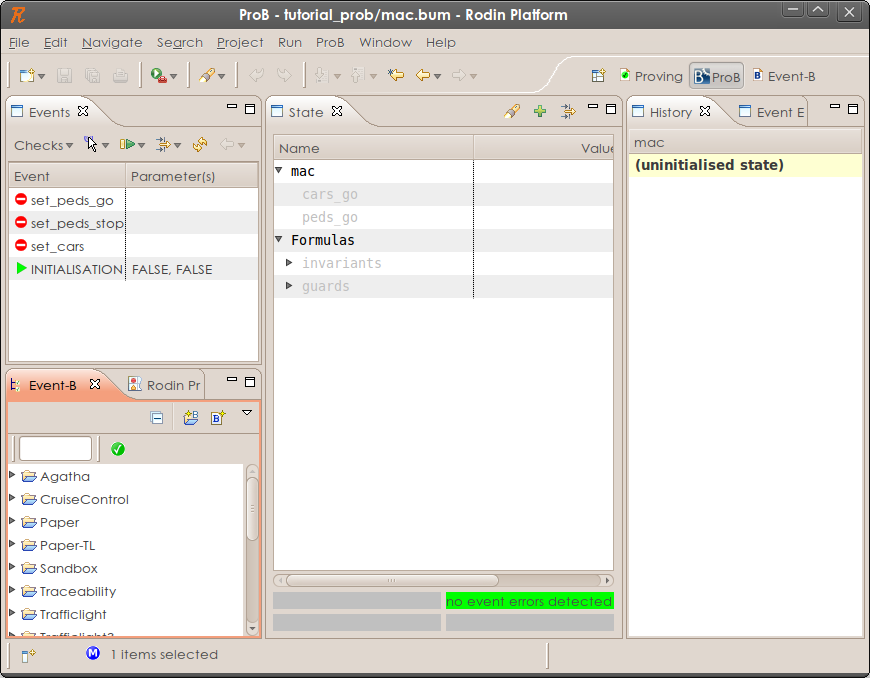
\includegraphics[]{img/tutorial/tut_03_prob_perspective.png}
	\caption{The ProB Perspective}
	\label{fig_tut_prob_perspective}
\end{center}
\end{figure}

\begin{figure}[!ht]
\begin{center}
	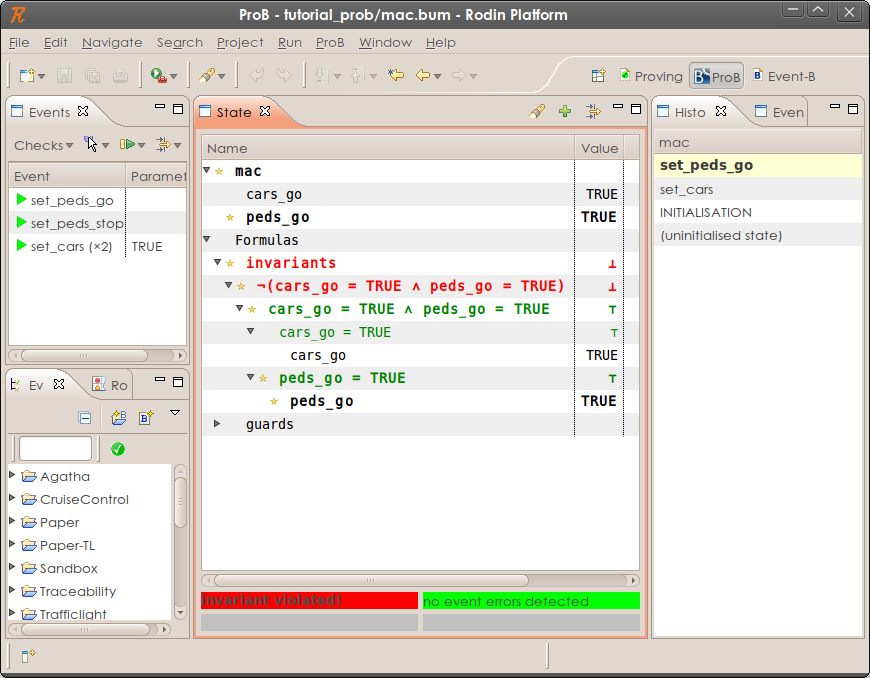
\includegraphics[]{img/tutorial/tut_03_prob_invariant_violation.png}
	\caption{An invariant violation, found by ProB}
	\label{tut_03_prob_invariant_violation}
\end{center}
\end{figure}


\subsection{The Final Traffic Light Model}
\label{tut_final_model}

\pencil{
\begin{description}
\MACHINE{mac}
\VARIABLES
	\begin{description}
		\Item{ cars\_go }
		\Item{ peds\_go }
	\end{description}
\INVARIANTS
	\begin{description}
		\nItemX{ inv1 }{ cars\_go \in  BOOL }
		\nItemX{ inv2 }{ peds\_go \in  BOOL }
		\nItemX{ inv3 }{ \lnot  (cars\_go = TRUE \land  peds\_go = TRUE) }
	\end{description}
\EVENTS
	\INITIALISATION
		\begin{description}
		\BeginAct
			\begin{description}
			\nItemX{ act1 }{ cars\_go :=  FALSE }
			\nItemX{ act2 }{ peds\_go :=  FALSE }
			\end{description}
		\EndAct
		\end{description}
	\EVT {set\_peds\_go}
		\begin{description}
		\WhenGrd
			\begin{description}
			\nItemX{ grd1 }{ cars\_go = FALSE }
			\end{description}
		\ThenAct
			\begin{description}
			\nItemX{ act1 }{ peds\_go :=  TRUE }
			\end{description}
		\EndAct
		\end{description}
	\EVT {set\_peds\_stop}
		\begin{description}
		\BeginAct
			\begin{description}
			\nItemX{ act1 }{ peds\_go :=  FALSE }
			\end{description}
		\EndAct
		\end{description}
	\EVT {set\_cars}
		\begin{description}
		\AnyPrm
			\begin{description}
			\ItemX{ new\_value }
			\end{description}
		\WhereGrd
			\begin{description}
			\nItemX{ grd1 }{ new\_value \in  BOOL }
			\nItemX{ grd2 }{ new\_value = TRUE \limp  peds\_go = FALSE }
			\end{description}
		\ThenAct
			\begin{description}
			\nItemX{ act1 }{ cars\_go :=  new\_value }
			\end{description}
		\EndAct
		\end{description}
\END
\end{description}
}


%%% Local Variables: 
%%% mode: latex
%%% TeX-master: "rodin-doc"
%%% End: 
